\documentclass[twocolumn]{IEEEtran}

\usepackage[ansinew]{inputenc} 
\usepackage{amsmath}
\usepackage{graphicx}
\usepackage{graphics}
\usepackage{hyperref}
\usepackage{longtable}               
\usepackage{fancyhdr}
\usepackage{times}
\usepackage{color}                   
\usepackage{makeidx}                 
\usepackage{cite}
\usepackage{float}
\setcounter{page}{1}


\begin{document}

\title{Identificaci�n de una planta de 3 Opams (sistema de tercer orden) utilizando la estructura param�trica ARMAX.}


\author{Autores \\ 
				Estrada Vidal, Jorge  \textcolor{blue}{jor1550g@gmail.com} \\
				Florian Chacon, Erick  \textcolor{blue}{erick.florian.uni@gmail.com} \\
				Giraldo Castillo, Oscar \textcolor{blue}{oscar.gi.cast@gmail.com} \\ 		
				\vspace{4 mm}
				Asesores: \\
				Ing. Rodriguez Bustinza, Ricardo \textcolor{blue}{robust@uni.edu.pe} \\ 	
				
				\vspace{8 mm}
				\emph{Universidad Nacional de Ingenier\'ia}
		}			

		
		
%\markboth{IEEE Trans...}{Murray and Balemi: ...}
\maketitle





\section{OBJETIVOS} %%%%%%%%%%%%%%%%%%%%%%%%%%%%%%%%%%%%%%%%%%%%%%%%%%%%%%%%%%%%%%%%%%%%%%%%%%%%%%%%%%%%%%%%%%%%%%%%%%%%%%%%%

\begin{itemize} \item Identificar el modelo de un planta de 3 Op-Amp?s a trav�s de la adquisici�n de datos y de la estructura param�trica ARMAX \end{itemize}

\section{MARCO TE�RICO}%%%%%%%%%%%%%%%%%%%%%%%%%%%%%%%%%%%%%%%%%%%%%%%%%%%%%%%%%%%%%%%%%%%%%%%%%%%%%%%

% ----------------------------------------------------------------------------------------------------
\subsection{Estructuras de modelos parametricos}
Las estructuras de modelos tambien conocidas como ``cajas negras'' quedan representadas por ejemplo, mediante una ecuaci�n lineal en diferencias dado por:

% ------------ Ecuacion numero 1 --------------
\begin{eqnarray}
\nonumber y \big(t\big) + a_{1} y \big(t-1\big) +...+ a_{ n_{a} } y \big(t- n_{a} \big) = \\
b_{1}  u_{t-1} +...+ b_{ n_{b} } y \big(t- n_{b} \big) +e \big(t\big) \label{eq:1}
\end{eqnarray}
% -------------- FIN DE ECUACION --------------

El termino de ruido blanco, e(t) aca ingresa como un error directo en la ecuacion en diferencias dada en ~\ref{eq:1}, a menudo es llamada ecuacion del modelo de error (estructura).\\

El vector que es llamado vector de parametros es el objetivo del estudio, es decir, encontrando dicho vector podemos conocer el modelo discreto y por ende el modelo continuo.

% ------------ Ecuacion numero 2 --------------
\begin{eqnarray}
 \theta = \big(
 \begin{array}{ccccccc}
 a_{1} & a_{2} & \cdots &  a_{ n_{a} } & b_{1} & \cdots &  b_{ n_{b} }
\end{array}
\big)  ^{T} \label{eq:2}
\end{eqnarray}
% -------------- FIN DE ECUACION --------------

Dentro de estas estructuras parametricas principales que nos proporcionan las herramientas del software de simulacion de Matlab y LabVIEW est�:\\

\paragraph{Estructura Parametrica ARX}
\paragraph{Estructura Parametrica ARMAX}
\paragraph{Estructura Parametrica OE (Output Error)}
\paragraph{Estructura Parametrica BJ (Box Jenkins)}

En este laboratorio, estudiaremos la segunda estructura que describiremos a continuaci�n:

% ----------------------------------------------------------------------------------------------------
\subsection{Estructura ARMAX}
El modelo ARMAX (AutoRegresive eXogenous Moving Average) es mas flexible describiendo la ecuacion de error como un ``promedio movil'', el ruido blanco puede ser representado por e(t), el modelo presenta la relacion de entrada y salida que puede ser descrita por una ecuacion en diferencia lineal en la forma.

% ------------ Ecuacion numero 3 --------------
\begin{eqnarray}
y\big(t\big) = \frac{B \big(q\big) }{A \big(q\big) } U \big(t\big)+ \frac{C \big(q\big) }{A \big(q\big) } e \big(t\big) \label{eq:3}
\end{eqnarray}
% -------------- FIN DE ECUACION --------------

Siendo su funci�n de transferencia:

% ------------ Ecuacion numero 4 --------------
\begin{eqnarray}
Y\big(z\big) = \frac{B \big(z\big) }{A \big(z\big) }  z^{-d}U \big(z\big)+ \frac{C \big(z\big) }{A \big(z\big) } E \big(z\big) \label{eq:4}
\end{eqnarray}
% -------------- FIN DE ECUACION --------------

\begin{figure}[h!]
	\centering % Requires \usepackage{graphicx}
 	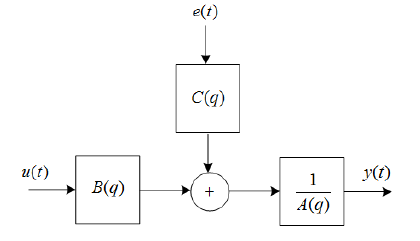
\includegraphics[height=4cm]{images/ARMAX_structure.png}
 	\caption{Estructura ARMAX.}
 	\label{fig:armax_structure}
\end{figure}

A continuaci�n presentamos un esquema b�sico del sistema analizado (ver Fig. ~\ref{fig:system_diagram}).\\

\begin{figure}[h!]
  \centering
    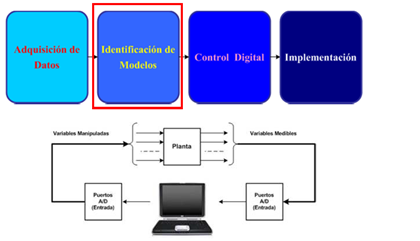
\includegraphics[height=4cm]{images/system_diagram.png}
  \caption{Esquema b�sico del sistema analizado}
  \label{fig:system_diagram}
\end{figure}

En donde el bloque etiquetado como planta contiene lo siguiente: (ver Fig. ~\ref{fig:system_proteus})

\begin{figure}[h!]
  \centering
    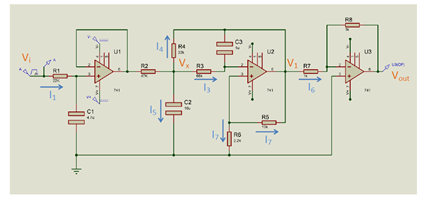
\includegraphics[height=4cm]{images/system_proteus.png}
  \caption{Esquema realizado en Proteus}
  \label{fig:system_proteus}
\end{figure}

Cuya simulaci�n obtenida en Proteus es la siguiente: (ver Fig. ~\ref{fig:simulation_proteus})

\begin{figure}[h!]
  \centering
    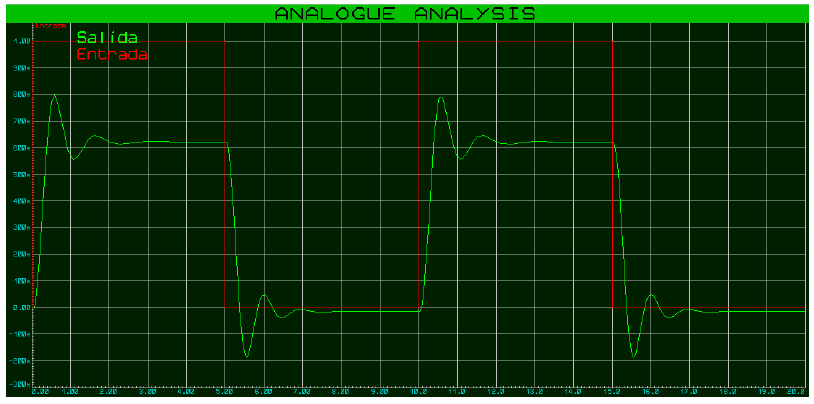
\includegraphics[height=4cm]{images/simulation_proteus.png}
  \caption{Respuesta de la planta a la funci�n Gate}
  \label{fig:simulation_proteus}
\end{figure}
 

\section{PRESENTACI�N DE RESULTADOSS} %%%%%%%%%%%%%%%%%%%%%%%%%%%%%%%%%%%%%%%%%%%%%%%%%%%%%%%%%%%%%%%%%%%%%%%%%%%%%%%%%%%%%%%%%%%%%%%%%%%%%%%%%%

Los resultados se obtuvieron mediante comandos de Matlab y por LabView los cuales estan incluidos en las 
carpetas ``graphics-matlabcommands'' 
, ``graphics-matlabident'' , ``labview-ident.vi''


\section{CONCLUSIONES} %%%%%%%%%%%%%%%%%%%%%%%%%%%%%%%%%%%%%%%%%%%%%%%%%%%%%%%%%%%%%%%%%%%%%%%%%%%%%%%%%%%%%%%%%%%%%%%%%%%%%%%%%%%%%%%%%%%%%%%%%

\begin{itemize}
\item Se debe estar consciente que el periodo de muestreo empleado en la adquisici�n de datos (usando DAQ) no debe cambiar al momento de realizar la identificaci�n debido a que al hacerlo pudimos notar que la se�al sufre una divisi�n en su frecuencia mientras m�s distante el tiempo de muestreo empleado sea del real. As� mismo cabe resaltar que nuestro $T_{s}=0.033...$, sin embargo, para labview basta con aproximarlo con $T_{s}=0.03$, de lo contrario nos encontraremos con errores propios del software.

\item Los modelos identificados con buena performance (mayor a 89%) se mimetizan cuando a todos ellos se les aplica una entrada gate llegando a asimilarse de forma muy cercana a la data experimental y te�rica. (ver Fig. ~\ref{gate_for_all_identified_models}).

\item Podemos observar que mientras las respuestas se mimetizan, las funciones de transferencia parecen cambiar tanto en orden como en coeficientes dependiendo de los par�metros usados en ARMAX. As� mismo, podemos observar que tanto Matlab como Labview resuelven los modelos ARMAX para los mismos par�metros, entradas y salidas de forma parecida (los coeficientes tienden a ser los mismos).


\item El tipo de entrada para la cual se puede obtener mayor caracter�stica del sistema es la se�al gate y step(en segundo lugar), y la menor es la rampa y seno es por ello que ante una entrada gate, nuestra estructura ARMAX identifica un modelo con alto performance respecto a otras entradas. Es por ellos que cuando comparamos a todos los modelos frente a nuestra salida experimental, las que los modelos identificados que m�s la mimetizan son los del producto del gate y step.

\item Las estructura ARMAX(1,1,1,1) o ARX pueden ser adecuadas para sistemas de primer orden, pero para el nuestro no lo es quedando comprobado en los graficos en los cuales comparamos diversas estructuras. 

\item No siempre la estructura de mayor orden determina un mayor performance, y as� lo hiciera se debe analizar el la eficiencia desde un punto de vista de desarrollo (computacional). 


\end{itemize}


\bibliographystyle{IEEE} %%%%%%%%%%%%%%%%%%%%%%%%%%%%%%%%%%%%%%%%%%%%%%%%%%%%%%%%%%%%%%%%%%%%%%%%%%%%%%%%%%%%%%%%%%%%%%%%%%%%%%%%%%%%%%%%%

\nocite{*}
\bibliographystyle{IEEE}

\begin{thebibliography}{1}

\bibitem{uno}
Ministerio de Salud, Per�
\newblock {\em REGISTRO NACIONAL DISCAPACIDAD EN CIFRAS}
\newblock CONADIS-INEI 2008

\bibitem{git}
bitbucket.org
\newblock {\em http://git-scm.com/}
\newblock 

\bibitem{bitbucket}
bitbucket.org
\newblock {\em https://bitbucket.org/jorgenro/proyecto-mecatronico}
\newblock Repositorio privado

\end{thebibliography}




\end{document}
